\section{Βελτιστοποίηση Μονοπατιού Κάλυψης Δωματίου}
\label{section:room_path_implementation}

Το τελευταίο και μεγαλύτερο τμήμα της εργασίας αυτής είναι η πλήρης κάλυψη κάθε δωματίου. Για να επιτευχθεί αυτό χρειάζεται να υπολογιστούν σημεία στα οποία θα κατευθυνθεί το ρομποτικό όχημα σαρώνοντας, έτσι, έμμεσα τον χώρο. Όλοι οι υπολογισμοί πραγματοποιούνται συναρτήσει των αισθητήρων. Υλοποιήθηκαν δύο διαφορετικές στρατηγικές, η στρατηγική ακολουθίας τοίχων και η στρατηγική ζιγκ ζαγκ. Η διαδικασία αυτή αποτελείται από τα παρακάτω βήματα:

\begin{itemize}
    \setlength\itemsep{-0.2em}
    \item Δειγματοληπτικός υπολογισμός σημείων κάλυψης
    \item Υπολογισμός βέλτιστης αλληλουχίας επίσκεψης των σημείων
    \item Υπολογισμός βέλτιστου προσανατολισμού σε κάθε σημείο
    \item Προσομοίωση κάλυψης του χώρου και διαγραφή περιττών σημείων
    \item Δημιουργία αλληλουχίας κόμβων ζιγκ-ζαγκ
\end{itemize}

\subsection{Δειγματοληπτικός υπολογισμός σημείων κάλυψης}
\label{subsection:nodes_sampling}

Αρχικά, πρέπει να εξαχθεί ένα σύνολο σημείων στα οποία πηγαίνοντας το όχημα θα έχει την δυνατότητα να καταγράψει προϊόντα, δηλαδή σημεία που βρίσκονται κοντά σε εμπόδια. Το πόσο κοντά, φυσικά, εξαρτάται από την ακτίνα των κεραιών RFID που φέρει το ρομπότ.

Η μέθοδος που υλοποιήθηκε εφαρμόζει ομοιόμορφη δειγματοληψία επαναληπτικά μεταβάλλοντας το βήμα της και αποθηκεύει όλα τα σημεία τα οποία βρίσκονται σε κοντινή απόσταση από τα γύρω εμπόδια. Το κέρδος με την χρήση πολλών διαφορετικών βημάτων είναι ότι αποθηκεύονται σημεία σε όλο τον ελεύθερο χώρο που μπορεί να επισκευτεί το ρομπότ ανεξαρτήτως της τοπολογίας του. 

Πρώτα υπολογίζονται η ελάχιστη και η μέγιστη τιμή των ακτίνων των διάφορων κεραιών που φέρει το ρομπότ. Μετά, επαναληπτικά σαρώνεται ολόκληρος ο χάρτης με κάποιο βήμα και κρατούνται όλα εκείνα τα σημεία που βρίσκονται στον ελεύθερο χώρο και απέχουν απόσταση από τα γύρω εμπόδια στο διάστημα $(step, 2*step]$. Θέτοντας αυτόν τον περιορισμό, σε κάθε επανάληψη σχηματίζεται μόλις μία σειρά σημείων εσωτερικά των εμποδίων και όχι περισσότερες, κάτι που οδηγεί σε μεγάλο πλεόνασμα σημείων μέσα στην ίδια επανάληψη. Το \autoref{fig:sampling_double_points_example} αποτελεί μια περίπτωση περισσότερων της μίας σειράς σημείων. Φυσικά, για να γίνει δεκτό ένα σημείο πρέπει οι κεραίες να είναι επαρκώς κοντά σε κάποιο εμπόδιο.


\begin{figure}[!htb]
    \centering
    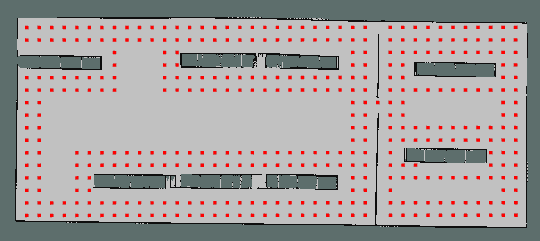
\includegraphics[width=0.8\textwidth]{./images/chapter5/sampling_double_points_example.png}
    \caption{Παράδειγμα Αποτυχίας Εύρεσης Σημείων}
    \label{fig:sampling_double_points_example}
\end{figure}


Το βήμα της δειγματοληψίας αρχίζει από τιμή ίση με μιάμιση φορά την ακτίνα του οχήματος, όσο δηλαδή και η ελάχιστη απόσταση που μπορεί να φτάσει το όχημα από τα εμπόδια για λόγους ασφαλείας και διπλασιάζεται σε κάθε επανάληψη μέχρι να γίνει μεγαλύτερο από την μέγιστη ακτίνα των κεραιών. Ένα τέτοιο παράδειγμα για τα σημεία με διαφορετικό βήμα δειγματοληψίας παρουσιάζεται στο \ref{fig:sampling_steps_examples}. Έτσι, όμως, θα υπάρχουν πολλά σημεία απ' όπου το ρομπότ θα σαρώσει τα ίδια εμπόδια, είναι δηλαδή περιττά. Επομένως, πρέπει να γίνει ένας τελικός έλεγχος εαν κάθε σημείο προσφέρει όντως στην κάλυψη, δίνοντας προτεραιότητα στα σημεία που προέκυψαν από την δειγματοληψία με τα μεγαλύτερα βήματα. Για κάθε σημείο υπολογίζονται τα εμπόδια που μπορούν να σαρωθούν από εκεί και εαν περισσότερα από το 90\% τους έχουν ήδη καλυφθεί από τα προηγούμενα, τότε αυτό απορρίπτεται. Σημειώνεται ότι τα σημεία που προέκυψαν από το μεγαλύτερο βήμα δειγματοληψίας κρατούνται όλα. Με τη μέθοδο αυτή εξασφαλίζεται ότι θα αποθηκευτούν τελικά τα λιγότερα δυνατά σημεία που καλύπτουν ολόκληρο τον χώρο. Ο αλγόριθμος περιγράφεται αναλυτικά στο \ref{alg:uniform_sampling}.


\begin{algorithm}[!htb]
\caption{Uniform Sampling}
\label{alg:uniform_sampling}
\begin{algorithmic}[1]
    \Function{uniformSampling}{brush, sensor\_range, resolution, robot\_radius}
    \State $nodes = [], step\_list = []$
    \State $min\_range = int(min(sensor\_range)/resolution)$
    \State $max\_range = int(max(sensor\_range)/resolution)$
    \State $step = int(1.5 * robot\_radius / resolution)$
    \While{$step <= max\_range$} 
        \State $temp\_nodes = []$
        \State $step\_list.append(step)$
        \State $indexes = np.where((brush > step)\ \&\ (brush <= 2*step)\ \&\ (brush <= max\_range))$
        \State $indexes = zip(*indexes)$
        \For{each $(x,y)$ in $indexes$}
            \If{not $x\ \%\ step$ and not $y\ \%\ step$}
                \State $temp\_nodes.append((x,y))$
            \EndIf
        \EndFor
        \State $step *= 2$
        \State $nodes.append(temp\_nodes)$
    \EndWhile
    \State $obstacles = numpy.zeros(brush.shape), final\_nodes = [], i = len(nodes) - 1$
    \While{$i >= 0$}
        \State $temp\_nodes = nodes[i]$
        \State \Comment{Check if new nodes override previous ones and delete them}
        \For{$point$ in $temp\_nodes$}
            \State $indexes = circularRayCastCoverage(point, ogm, max\_range,$ \par
            \hskip \algorithmicindent $360, 0, 0, True)$
            \If{not $len(indexes)$}
                \State continue
            \ElsIf{$i == len(nodes) - 1$}
                \State $obstacles[zip(*indexes)] = 1$
                \State $final\_nodes.append(point)$
            \Else
                \State $temp = obstacles[zip(*indexes)]$
                \State $p = len(np.where(temp > 0)[0]) / len(indexes)$
                \If{$p<0.9$}
                    \State $final\_nodes.append((x,y))$
                    \State $obstacles[zip(*indexes)] = 1$
                \EndIf
            \EndIf
        \EndFor
        \State $i -= 1$
    \EndWhile
    \State \Return $final\_nodes, step\_list$
\end{algorithmic}
\end{algorithm}


\begin{figure}
     \centering
     \begin{subfigure}[b]{\textwidth}
         \centering
         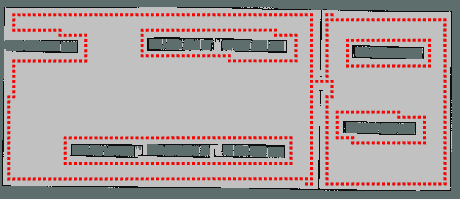
\includegraphics[width=0.8\textwidth]{./images/chapter5/warehouse_4_sampling_steps_1.png}
         \label{fig:warehouse_4_sampling_steps_1}
     \end{subfigure}
     \hfill
     \begin{subfigure}[b]{\textwidth}
         \centering
         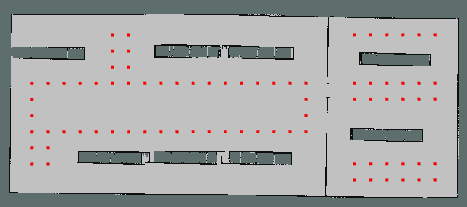
\includegraphics[width=0.8\textwidth]{./images/chapter5/warehouse_4_sampling_steps_2.png}
         \label{fig:warehouse_4_sampling_steps_2}
     \end{subfigure}
     \hfill
     \begin{subfigure}[b]{\textwidth}
         \centering
         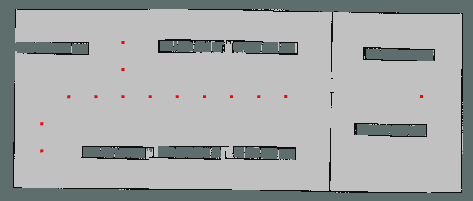
\includegraphics[width=0.8\textwidth]{./images/chapter5/warehouse_4_sampling_steps_3.png}
         \label{fig:warehouse_4_sampling_steps_3}
     \end{subfigure}
    \caption{Δειγματοληψία με διάφορα βήματα}
    \label{fig:sampling_steps_examples}
\end{figure}


Αντίθετα, εαν γίνει χρήση σταθερού βήματος δειγματοληψίας είναι πολύ πιθανό να προκύψουν περιοχές χωρίς σημεία πράγμα που σημαίνει αποτυχία πλήρους κάλυψης του χώρου, όπως φαίνεται και στο σχήμα \ref{fig:wrong_sampling_example}.


\begin{figure}[!htb]
    \centering
    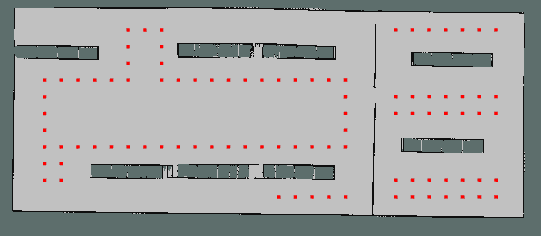
\includegraphics[width=0.8\textwidth]{./images/chapter5/range_2_get_only_in_second_half.png}
    \caption{Παράδειγμα Αποτυχίας Εύρεσης Σημείων}
    \label{fig:wrong_sampling_example}
\end{figure}




\subsection{Υπολογισμός βέλτιστης αλληλουχίας επίσκεψης των σημείων}
\label{subsection:node_sequence_optimization}

Στην συνέχεια, τα σημεία αυτά χωρίζονται στα διάφορα δωμάτια και υπολογίζεται η βέλτιστη αλληλουχία των σημείων ανά δωμάτιο. Η διαδικασία αυτή έχει τα παρακάτω βήματα.

\begin{itemize}
    \setlength\itemsep{-0.2em}
    \item Διαχωρισμός σημείων σε δωμάτια
    \item Hill Climbing σε συνδιασμό με τον αλγόριθμο κοντινότερου γείτονα
    \item Προσθήκη των πορτών εισόδου και εξόδου του δωματίου στην αλληλουχία
    \item RRHC με τις πόρτες σταθερές στις άκρες της αλληλουχίας
\end{itemize}

Ο διαχωρισμός των κόμβων σε δωμάτια πραγματοποιείται χωρίζοντας το OGM σε ασύνδετους χώρους, δηλαδή προσθέτοντας τοίχους εκεί που υπάρχουν οι πόρτες και χρησιμοποιώντας μια παραλλαγή του αλγορίθμου brushfire, την \emph{pointBrushfire}. 

Οι πόρτες του χώρου είναι ήδη γνωστές ενώ τα κοντινότερα εμπόδια τους, δηλαδή οι δύο τοίχοι υπολογίζονται από τον αλγόριθμο \emph{closestObstacleBrushfire} \ref{alg:closestObstacleBrushfire}. Στη συνέχεια, υπολογίζεται η νοητή ευθεία του τοίχου, δηλαδή η ευθεία της κάθε πόρτας στο OGM και προστίθεται τοίχος, δηλαδή τα σημεία αυτά τίθονται ίσα με $100$ στο νέο OGM. Η συνάρτηση αυτή παρουσιάζεται στο \ref{alg:door_closure}.

\begin{algorithm}[!htb]
\caption{Door Closure}
\label{alg:door_closure}
\begin{algorithmic}[1]
    \Function{doorClosure}{doors, ogm}
    \State $filled\_ogm = numpy.copy(ogm)$
    \For{$door$ in $doors$}
        \State $ob = closestObstacleBrushfire(door, ogm)$
        \State Find obstacle points' line
        \State Set points of line equal to $100$ in $filled\_ogm$
    \EndFor
    \State \Return $filled\_ogm$
\end{algorithmic}
\end{algorithm}


Έπειτα, με την χρήση brushfire με αρχή τους κόμβους κάθε δωματίου από την προηγούμενη διαδικασία εξαγωγής χρήσιμων σημείων από το GVD \ref{subsection:find_room_nodes} και το διαχωρισμένο σε δωμάτια OGM χωρίζονται οι κόμβοι προσπέλασης σε δωμάτια.

Στη συνέχεια, για κάθε δωμάτιο υπολογίζεται μια βέλτιστη αλληλουχία. Τα σημεία ταξινομούνται σύμφωνα με τις συντεταγμένες τους $(x,y)$ και στη συνέχεια χρησιμοποιείται μια παραλλαγή του HC που αξιοποιεί το γεγονός ότι η δειγματοληψία των σημείων έχει πραγματοποιηθεί με συγκεκριμένα βήματα. Αυτό σημαίνει ότι τα σημεία που είναι πολύ κοντά μεταξύ τους, θα έχουν απόσταση ίση με ένα από τα διάφορα βήματα, τα οποία έχουν αποθηκευτεί στο $step\_list$ στον αλγόριθμο \ref{alg:uniform_sampling}. Έτσι, υπολογίζεται μια αλληλουχία με βάση εαν τα σειριακά σημεία έχουν μεταξύ τους απόσταση ίση με τα βήματα της δειγματοληψίας. Εαν δεν υπάρχει τέτοιο σημείο, τότε προστίθεται στην σειρά το κοντινότερο δυνατό, χρησιμοποιείται, δηλαδή, και η προσέγγιση του κοντινότερο γείτονα. Ο αλγόριθμος που περιγράφει αυτή την διαδικασία παρουσιάζεται στο \ref{alg:step_hillclimb}.



\begin{algorithm}[!htb]
\caption{Step Hill Climb}
\label{alg:step_hillclimb}
\begin{algorithmic}[1]
    \Function{stepHillClimb}{distances, epochs, steps}
    \State $length = distances.shape[0]$
    \State $best = range(length)$
    \State Set $best\_score$ equal to the length of route $best$
    \State $iter = 0$
    \For{$i$ in $range(length-2)$}
        \If{$iter >= epochs$}
            \State break
        \EndIf
        \State $minimum = distances[best[i]][best[i+1]]$
        \If{$minimum <= min(steps)$}
            \State continue
        \Else
            \State Find point $index$ closest to point $i$
            \State $best[i+1], best[index] = best[index], best[i+1]$
            \State Set $best\_score$ equal to the length of route $best$
        \EndIf
    \EndFor
    \State \Return $best, best\_score, iter$
\end{algorithmic}
\end{algorithm}

Στη συνέχεια, προστίθενται και οι πόρτες εισόδου και εξόδου στην αρχή και στο τέλος αντίστοιχα της υπολογισμένης αλληλουχίας. Μάλιστα, για την περαιτέρω βελτίωση της, πραγματοποιείται μια εσωτερική κυκλική περιστροφή των σημείων, έτσι ώστε το δεύτερο σημείο να είναι το κοντινότερο από την πόρτα εισόδου που είναι το πρώτο σημείο. Αυτή είναι μια λογική μεταβολλή η οποία βελτιώνει την συνολική απόσταση του μονοπατιού χωρίς την χρήση σύνθετων αλγορίθμων.

Τέλος, εφαρμόζεται ο RRHC αλγόριθμος με σταθερά άκρα τις πόρτες εισόδου και εξόδου στο δωμάτιο. Μετά από πειραματισμούς στο πλήθος των επαναλήψεων του RRHC με τιμές 1000, 2000 και 5000 φορές επί το πλήθος των σημείων του δωματίου, προέκυψε ότι ιδανικότερος αριθμός είναι οι 2000 επί πλήθος των σημείων του δωματίου. Είναι ένας αριθμός που φέρει πολύ καλά αποτελέσματα χωρίς να απαιτεί σημαντικό χρόνο υπολογισμών. Ο RRHC αναλύεται στο \ref{alg:rrhc}.


Ένα παράδειγμα της προόδου του μήκους της αλληλουχίας των διάφορων δωματίων ενός χάρτη σε κάθε ένα από τα τέσσερα στάδια επεξεργασίας παρουσιάζεται στον επόμενο πίνακα \ref{tab:room_path_length_stages_optimization} και στα σχήματα \ref{fig:wall_follow_optimization_example}. Η μελέτη πραγματοποιήθηκε στο το OGM του σχήματος \ref{fig:wf_opt_ogm}, πάνω στο οποίο εμφανίζεται και με κόκκινους αριθμούς η σειρά των δωματίων. Η σειρά επίσκεψης των σημείων κάθε δωματίου οπτικοποιείται με την εναλλαγή χρωμάτων ανά δωμάτιο. Το όχημα θα εκκινεί από τα σκούρα σημεία και θα κατευθύνεται στα πιο ανοικτόχρωμα, καταλήγοντας στα άσπρα.


\begin{table}[H]
    \begin{center}
        \caption{Βελτίωση μήκους διαδρομής ανά στάδιο επεξεργασίας}
        \label{tab:room_path_length_stages_optimization}
        \begin{tabular}{|>{\columncolor[gray]{0.8}} c | c | c | c | c | c | c |}
        \hline
        \rowcolor{gray}
        Stages & room 1 & room 2 & room 3 & room 4 & room 5 & room 6 \\
        \hline
        sort & 14719 & 4711 & 5398 & 4699 & 4443 & 2633 \\ 
        \hline
        stepHC & 3951 & 1494 & 1049 & 945 & 1275 & 1024 \\
        \hline
        adding doors & 4554 & 1524 & 1060 & 1212 & 1283 & 1056 \\ 
        \hline
        RRHC & 3761 & 1344 & 935 & 1032 & 1131 & 944 \\ 
        \hline
        \end{tabular}
    \end{center}
\end{table}

\begin{figure}
    \centering
    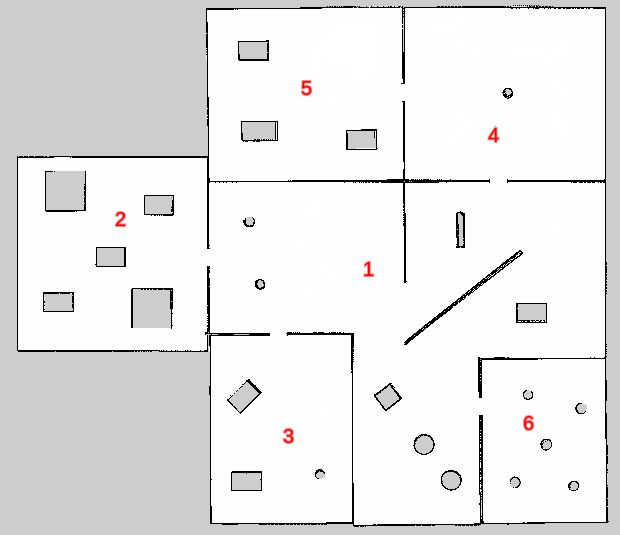
\includegraphics[width=0.5\textwidth]{./images/chapter5/wf_opt_ogm.png}
    \caption{Περιβάλλον ελέγχου διαδικασίας υπολογισμού μονοπατιού}
    \label{fig:wf_opt_ogm}
\end{figure}



\begin{figure}[!htb]
     \centering
     \begin{subfigure}[b]{0.5\textwidth}
         \centering
         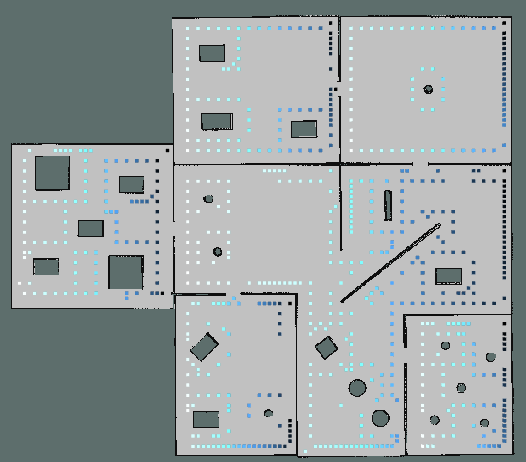
\includegraphics[width=0.9\textwidth]{./images/chapter5/wf_optimization_1_sorted.png}
         \label{fig:wf_optimization_1_sorted}
         \caption{sort}
     \end{subfigure}%
    %  \hfill
     \begin{subfigure}[b]{0.5\textwidth}
         \centering
         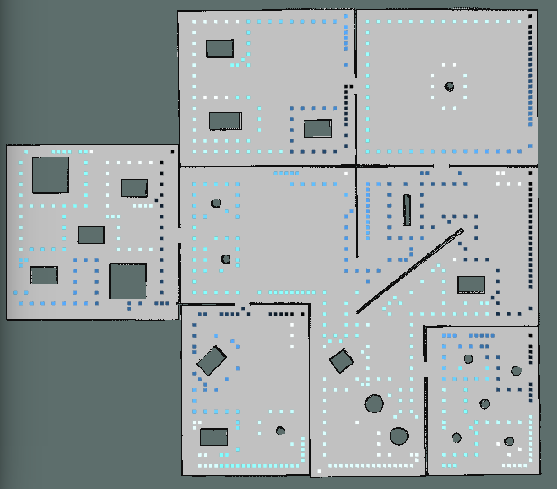
\includegraphics[width=0.9\textwidth]{./images/chapter5/wf_optimization_2_stepHC.png}
         \label{fig:wf_optimization_2_stepHC}
         \caption{stepHC}
     \end{subfigure}
     \hfill
     \begin{subfigure}[b]{0.5\textwidth}
         \centering
         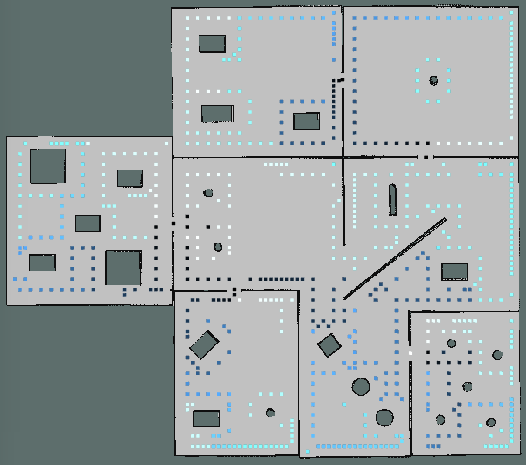
\includegraphics[width=0.9\textwidth]{./images/chapter5/wf_optimization_3_added_doors.png}
         \label{fig:wf_optimization_3_added_doors}
         \caption{adding doors}
     \end{subfigure}%
    %  \hfill
     \begin{subfigure}[b]{0.5\textwidth}
         \centering
         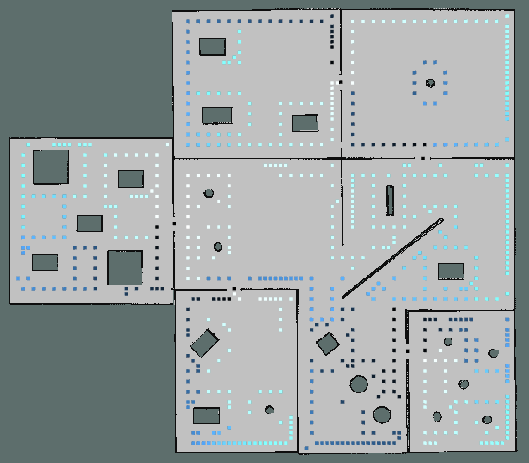
\includegraphics[width=0.9\textwidth]{./images/chapter5/wf_optimization_4_rrhc.png}
         \label{fig:wf_optimization_4_rrhc}
         \caption{RRHC}
     \end{subfigure}
    \caption{Στάδια βελτίωσης μονοπατιού}
    \label{fig:wall_follow_optimization_example}
\end{figure}



\subsection{Υπολογισμός βέλτιστου προσανατολισμού σε κάθε σημείο}
\label{subsection:find_pose}

Αφότου βρεθεί το σύνολο των σημείων για την πλήρη κάλυψη του χώρου, χρειάζεται να υπολογιστεί και η βέλτιστη γωνία του ρομπότ σε κάθε θέση. Άλλωστε, η ακριβής θέση του οχήματος στον διδιάστατο χώρο αποτελείται από τρεις μεταβλητές, δύο για την θέση και μία για τον προσανατολισμό. Τα κριτήρια επιλογής του προσανατολισμού είναι δύο. Το πρώτο είναι οι αισθητήρες να καλύπτουν όσο το δυνατόν περισσότερη επιφάνεια εμποδίων και το δεύτερο η γωνιακή μετατόπιση ανάμεσα στον τρέχοντα προσανατολισμό και το επόμενο σημείο να είναι η ελάχιστη δυνατή. Αυτά μας εξασφαλίζουν όσο το δυνατόν μεγαλύτερη κάλυψη του χώρου και ελαχιστοποίηση της χρονικής διάρκειας της διαδικασίας αντίστοιχα. Για τον λόγο αυτό δημιουργήθηκε μια συνδιαστική συνάρτηση των δύο αυτών παραμέτρων με την μέθοδο motor schema, όπου λαμβάνονται υπόψη και οι δύο παράμετροι με κάποιο βάρος. Η μέθοδος υπολογισμού των βαρών αυτών παρουσιάζεται στο τέλος της υποενότητας.

Πρώτα αναλύεται η διαδικασία επιλογής κάθε γωνίας στροφής. Για κάθε σημείο στόχο εξετάζονται όλες οι γωνίες μία προς μία με βήμα 10 μοιρών και κρατείται αυτή που δίνει την βέλτιστη τιμή της συνάρτησης του motor schema, η οποία είναι η παρακάτω.

\[eval = obstacle\_weight * \frac{len(covered\_obstacles)}{len(obstacles)} + rotation\_weight * \frac{180 - next\_rotation}{180}\]

Ο πρώτος όρος περιέχει το πλήθος των εμποδίων που καλύπτονται από την εν λόγω γωνία και ο δεύτερος περιέχει τη γωνιακή στροφή προς το επόμενο σημείο στόχο. Και οι δύο είναι κανονικοποιημένοι, έτσι ώστε οι τιμές να περιορίζονται στο εύρος $[0,1]$ και το $1$ να αντιστοιχεί στο βέλτιστο επιμέρους αποτέλεσμα. 

Σε κάθε σημείο, όμως, δεν αποθηκεύεται μόνο μια γωνία αλλά μπορούν και περισσότερες μέχρι να έχει συνολικά καλυφθεί το περισσότερο τμήμα των γύρω εμποδίων, δηλαδή ένα ποσοστό μεγαλύτερο του 50\%. Μετά από ορισμένες δοκιμές βρέθηκε ότι το όριο του 60\% προσφέρει καλή συνολική κάλυψη του χώρου. Mεγαλύτερα όρια, όπως τα 75\% και 80\%, οδηγούν σε αποθήκευση πολλών περιττών θέσεων - στόχων χωρίς βελτίωση στην συνολική τελική κάλυψη του χώρου, ενώ το μικρότερο όριο 50\% οδηγεί σε μείωση της κάλυψης. Συνεπώς, για κάθε σημείο αποθηκεύονται οι καλύτερες γωνίες εως ότου έχει καλυφθεί τουλάχιστον το 60\% των κοντινών εμποδίων. Το ποσοστό είναι φαινομενικά μικρό, ωστόσο εξαιτίας της κοντινής απόστασης μεταξύ των σημείων στόχων οδηγεί σε θεμιτά αποτελέσματα. 

Αυτό το κατώφλι χρησιμοποιήθηκε για τις περιπτώσεις που υπάρχουν περισσότερα του ενός εμπόδια στην γύρω περιοχή και το όχημα φέρει μικρό αριθμό αισθητήρων, για παράδειγμα έναν. Τότε εαν αποθηκευτεί ένας μόνο στόχος, είναι πολύ πιθανό να μην σαρωθεί σημαντικό τμήμα των εμποδίων. Με την πολλαπλή αποθήκευση γωνιών σε κάθε σημείο εξασφαλίζεται η καλύτερη δυνατή κάλυψη της κάθε περιοχής. Ο αλγόριθμος αυτός παρουσιάζεται αναλυτικά στο \ref{alg:find_best_yaw}.  

\begin{algorithm}[!h]
\caption{Find Best Yaw}
\label{alg:find_best_yaw}
\begin{algorithmic}[1]
    \Function{findBestYaw}{node, next\_node, obstacle\_weight, rotation\_weight, sensor\_range, resolution}
        \State $yaw = []$
        \State $yaw\_between\_nodes = math.degrees(math.atan2(next\_node[1]-node[1], next\_node[0]-node[0]))$
        \State $steps = int(max(sensor\_range) / resolution)$
        \State Fill $obstacles$ with indexes of nearby obstacles at range $steps$
        \State $found = 0$
        \While{$found < 0.6 * len(obstacles)$ and $len(obstacles)$}
            \State $best\_evaluation = 0$, $best\_yaw = 0$, $best\_found = 0$, $best\_covered\_obstacles = []$
            \For{each angle $angle$ in $[-180, 180]$}
                \State Check covered nearby obstacles $covered\_obstacles$
                \State $next\_rotation = abs(angle - yaw\_between\_nodes)$
                \State Evaluate candidate angle
                \If{$angle$ is better than current best}
                    \State $best\_evaluation = angle$'s evaluation
                    \State $best\_yaw = angle$
                    \State $best\_found = len(covered\_obstacles)$ 
                    \State $best\_covered\_obstacles = covered\_obstacles$
                \EndIf
            \EndFor
            \State $found += best\_found$
            \State Discard $best\_covered\_obstacles$ from $obstacles$
        \EndWhile
        \State \Return $best\_yaw$
\end{algorithmic}
\end{algorithm}



Τέλος, η διαδικασία αυτή υλοποιήθηκε σε έναν συγκεκριμένο χάρτη με πέντε διαφορετικούς συνδιασμούς βαρών, ώστε να μελετηθεί η επιρροή τους και να επέλθει η τελική μέθοδος επιλογής τους στην προηγούμενη συνάρτηση. Μελετήθηκαν η εκτίμηση της κάλυψης του χώρου, η πραγματική κάλυψη του και ο χρόνος της και τα αποτελέσματα παρουσιάζονται στους επόμενους δύο πίνακες \ref{tab:motor_schema_weights_side_antennas}, \ref{tab:motor_schema_weights_front_back_antennas} για διαφορετικούς αισθητήρες. Στην πρώτη περίπτωση οι κεραίες είναι τοποθετημένες στα πλάγια του οχήματος, ενώ στην δεύτερη στο μπροστά και το πίσω μέρος του. 

\begin{table}[H]
    \centering
    \begin{tabular}{|>{\columncolor[gray]{0.8}} c | >{\columncolor[gray]{0.8}} c  | c | c | c |}
        \hline
             Obstacle W.  & Rotation W. & Εκτίμηση  & Πραγματική Κάλυψη & Χρόνος  \\
             \hline
             $4$ & $1$ & $85.49$ \% & $87.43$ \% & 71.6 min \\
             $2$ & $1$ & $85.80$ \% & $85.95$ \% & 71.2 min \\
             $1$ & $1$ & $85.04$ \% & $86.78$ \% & 66 min \\
             $1$ & $2$ & $83.16$ \% & $86.20$ \% & 59.5 min \\
             $1$ & $4$ & $83.16$ \% & $86.74$ \% & 76.6 min \\
        \hline
    \end{tabular}
    \caption{Εκτίμηση Βαρών Motor Schema με Κεραίες στα Πλάγια}
    \label{tab:motor_schema_weights_side_antennas}
\end{table}

\begin{table}[H]
    \centering
    \begin{tabular}{|>{\columncolor[gray]{0.8}} c | >{\columncolor[gray]{0.8}} c  | c | c | c |}
        \hline
             Obstacle W.  & Rotation W. & Εκτίμηση  & Πραγματική Κάλυψη & Χρόνος  \\
             $4$ & $1$ & $85.95$ \% & $83.03$ \% & 76 min \\
             $2$ & $1$ & $85.34$ \% & $83.61$ \% & 73.7 min \\
             $1$ & $1$ & $84.85$ \% & $80.58$ \% & 66.4 min \\
             $1$ & $2$ & $83.29$ \% & $84.38$ \% & 98.18 min \\
             $1$ & $4$ & $82.81$ \% & $85.41$ \% & 122.1 min \\
        \hline
    \end{tabular}
    \caption{Εκτίμηση Βαρών Motor Schema με Κεραίες Μπροστά και Πίσω}
    \label{tab:motor_schema_weights_front_back_antennas}
\end{table}

Τα συμπεράσματα που προκύπτουν είναι ότι ο χρόνος ελαχιστοποιείται όταν το βάρος της γωνιακής κίνησης είναι λίγο μεγαλύτερο από το βάρος της κάλυψης, αλλά όταν γίνει πολύ μεγαλύτερο, με αναλογία πάνω από δύο προς ένα, τότε δημιουργούνται πολλά περιττά σημεία προσπέλασης αυξάνοντας ριζικά τον χρόνο. Αντίθετα, η χρήση μεγαλύτερου βάρους στο ποσοστό κάλυψης δεν βελτιώνει την συνολική κάλυψη του χώρου, αλλά αυξάνει τον συνολικό χρόνο της διαδικασίας. Συνεπώς, τα βάρη και αυτά με την σειρά τους εξαρτώνται άμεσα από την θέση των κεραιών και, μάλιστα, όσο πιο κεντρικά είναι αυτές, τόσο μεγαλύτερο βάρος πρέπει να δίνεται στο ποσοστό κάλυψης, ενώ όσο πιο πλάγια είναι τόσο πρέπει να αυξάνεται το βάρος της περιστροφής. Στην προκειμένη περίπτωση κέντρο είναι η διάμετρος του οχήματος που διέρχεται από το μπροστινό του μέρος. Οι συντελεστές θα κυμαίνονται στο πεδίο $[1,2]$, όπου και βελτιστοποιείται η διαδικασία. Οι ακριβείς συναρτήσεις που χρησιμοποιήθηκαν παρουσιάζονται στην συνέχεια.

\[obstacle\_weight = 1 + \frac{90 - theta}{90}\]
\[rotation\_weight = 2 - \frac{90 - theta}{90}\]
Όπου $theta = mean(sensor\_direction)$. Στόχος είναι, δηλαδή, η κεραία να κοιτάει όσο πιο κεντρικά γίνεται το κάθε εμπόδιο, εξασφαλίζοντας την καλύτερη δυνατή κάλυψη. Σημειώνεται ότι αρχικά η γωνία κατεύθυνσης κάθε αισθητήρα μετασχηματίζεται στο πεδίο $[0,90]$ για την ευκολότερη ανάλυση των δεδομένων.

Τα συμπεράσματα αυτά μπορούν να γίνουν κατανοητά και από τις επόμενες εικόνες \ref{fig:different_yaw_examples}. Στις δύο επάνω εικόνες οι κεραίες είναι τοποθετημένες στο μπροστά και το πίσω μέρος του οχήματος. Η εμπρός κατεύθυνση του οχήματος φαίνεται από το μπλε βέλος. Είναι προτιμότερο το όχημα να μην κοιτάει απευθείας τα εμπόδια, αλλά να έχει μια ελαφριά κλίση προς τον επόμενο στόχο, καλύπτοντας όμως σημαντικό τμήμα του τοίχου. Έτσι, μετά τη σάρωση θα χρειαστεί να πραγματοποιήσει μικρότερη περιστροφική κίνηση για να φτάσει στον επόμενο στόχο. Αντίθετα, στις δύο κάτω εικόνες οι κεραίες είναι τοποθετημένες στα πλάγια μέρη του οχήματος. Στην περίπτωση αυτή είναι προτιμότερο το όχημα να κοιτάει ακριβώς προς τον επόμενο στόχο. Έτσι, καλύπτει σταθερά τα εμπόδια κατά την μετακίνηση του, χωρίς να αποκλίνει από το μονοπάτι πλοήγησης του. Αυτή μάλιστα είναι η καλύτερη δυνατή τοποθέτηση των κεραιών, διότι το όχημα κινείται συνεχώς πάνω στην ευθεία μεταξύ των διαδοχικών στόχων. Με τη μέθοδο αυτή, λοιπόν, αποφεύγονται οι περιττές περιστροφικές κινήσεις και εξοικονομείται σημαντικός χρόνος και ενέργεια.


\begin{figure}[!htb]
     \centering
     \begin{subfigure}[b]{0.5\textwidth}
         \centering
         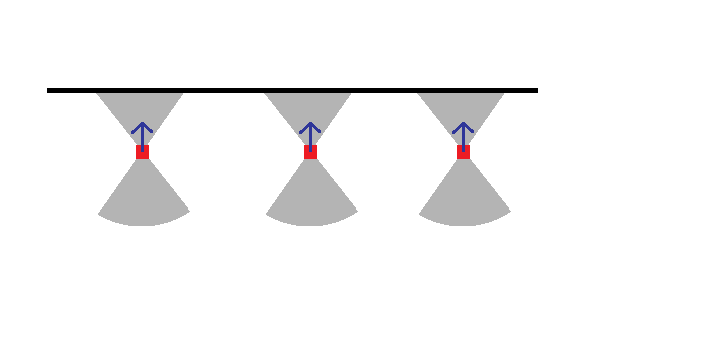
\includegraphics[width=0.9\textwidth]{./images/chapter5/set_one_front.png}
         \label{fig:set_one_front}
     \end{subfigure}%
     \begin{subfigure}[b]{0.5\textwidth}
         \centering
         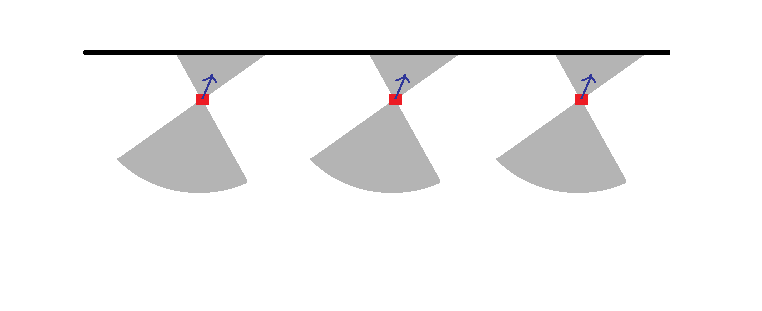
\includegraphics[width=0.9\textwidth]{./images/chapter5/set_two_front.png}
         \label{fig:set_two_front}
     \end{subfigure}
     \hfill
     
     \begin{subfigure}[b]{0.5\textwidth}
         \centering
         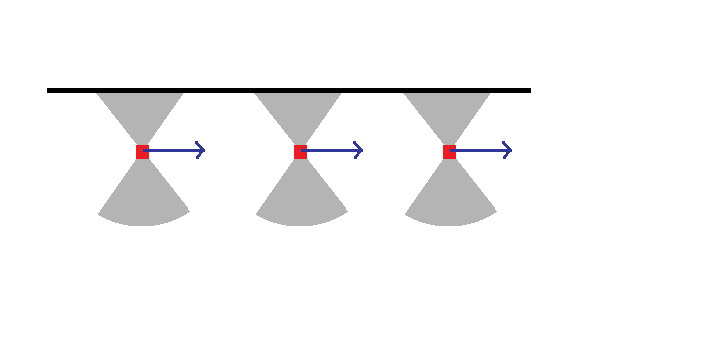
\includegraphics[width=0.9\textwidth]{./images/chapter5/set_one_side.png}
         \label{fig:set_one_side}
     \end{subfigure}%
    %  \hfill
     \begin{subfigure}[b]{0.5\textwidth}
         \centering
         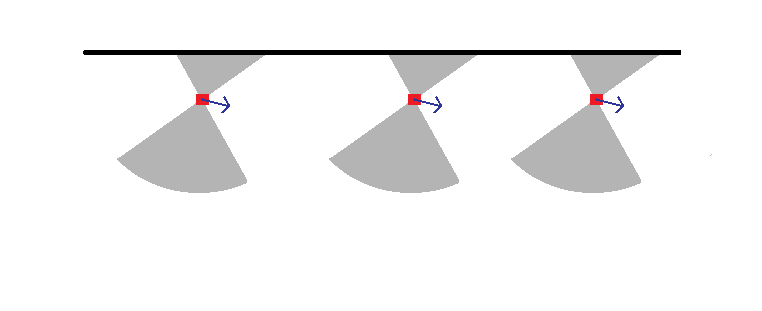
\includegraphics[width=0.9\textwidth]{./images/chapter5/set_two_side.png}
         \label{fig:set_two_side}
     \end{subfigure}
    \caption{Παραδείγματα διαφορετικών προσανατολισμών}
    \label{fig:different_yaw_examples}
\end{figure}


\begin{algorithm}[!htb]
\caption{Find Weights}
\label{alg:find_weights}
\begin{algorithmic}[1]
    \Function{findWeights}{sensor\_number, sensor\_direction, sensor\_fov}
        \State $angles = []$
        \For{$s$ in $range(sensor\_number)$}
            \State $theta = sensor\_direction[s]$
            \State Transform $theta$ to range $[0,90]$
            \State $angles.append((90-theta)/90)$
        \EndFor
        \State $obstacle\_weight = 1 + mean(angles)$
        \State $rotation\_weight = 2 - mean(angles)$
        \State \Return $obstacle\_weight, rotation\_weight$
\end{algorithmic}
\end{algorithm}



\subsection{Προσομοίωση κάλυψης του χώρου και διαγραφή περιττών σημείων}
\label{subsection:node_elimination}

Τελευταίο βήμα της δημιουργίας της πρώτης στρατηγικής πλοήγησης είναι η εκ των προτέρων εκτίμηση της κάλυψης του χώρου και η διαγραφή των στόχων που είναι περιττοί στην όλη διαδικασία. Η εκτίμηση της κάλυψης πραγματοποιείται προσομοιώνοντας τη μέτρηση των αισθητήρων του οχήματος για κάθε στόχο της ακολουθίας. Με τον τρόπο αυτό αποθηκεύονται σε ένα OGM τα σημεία τα οποία πρόκειται να καλυφθούν. Αυτή είναι η απλή περίπτωση με την οποία μπορεί να υπολογιστεί και το ποσοστό κάλυψης των εμποδίων του χώρου, όπως και έγινε στα πειράματα των πινάκων  \ref{tab:motor_schema_weights_side_antennas} και \ref{tab:motor_schema_weights_front_back_antennas}. Σημειώνεται ότι η κάλυψη αυτή είναι μια εκτίμηση, καθώς η πλοήγηση του οχήματος δεν περιλαμβάνεται στο σημείο αυτό με αποτέλεσμα να μην λαμβάνονται υπόψη οι ενδιάμεσες κινήσης μετάβασης από το κάθε σημείο στο επόμενο. Μάλιστα, η τελική πραγματική κάλυψη θα είναι, θεωρητικά, μεγαλύτερη της εκτίμησης.

Ένα παράδειγμα εκτίμησης κάλυψης παρουσιάζεται στο σχήμα \ref{fig:coverage_estimation_ogm_example}, όπου φαίνονται με διάφορες αποχρώσεις του μπλε τους στόχους και με σκούρο γκρι την περιοχή που εκτιμάται ότι θα καλύψει το όχημα από όλα τα σημεία. Επίσης, οπτικοποιείται και η σειρά προσπέλασης, η οποία εκκινεί για κάθε δωμάτιο από τα πιο σκούρα σημεία και κατευθύνεται στα πιο ανοικτόχρωμα, καταλήγοντας στα λευκά.

\begin{figure}[!htb]
    \centering
    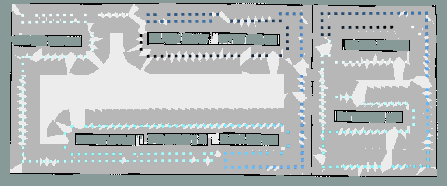
\includegraphics[width=0.9\textwidth]{./images/chapter5/warehouse_4_wall_follow_a_priori_coverage_085_cover_first_weights_2_1_multi_yaw_060.png}
    \caption{Παράδειγμα Πεδίου Εκτίμησης Κάλυψης}
    \label{fig:coverage_estimation_ogm_example}
\end{figure}

Αντίθετα, η διαγραφή σημείων προϋποθέτει τον έλεγχο κάθε φορά των εμποδίων που πρόκειται να καλυφθούν. Εαν το μεγαλύτερο ποσοστό τους είναι ήδη καλυμμένο, τότε το σημείο αυτό είναι περιττό για την μελέτη αυτή. Στόχος είναι να καλυφθεί όσο το δυνατό μεγαλύτερη επιφάνεια εμποδίων, δηλαδή ένα ποσοστό που πλησιάζει το 100\%. Μετά από ορισμένες δοκιμές βρέθηκε ότι το όριο του 85\% προσφέρει καλή συνολική κάλυψη του χώρου. Η χρήση μεγαλύτερων ορίων, όπως τα 90\% και 95\%, οδηγεί σε αποθήκευση πολλών περιττών θέσεων - στόχων χωρίς βελτίωση στην συνολική τελική κάλυψη του χώρου, ενώ το μικρότερο όριο 80\% οδηγεί σε μείωση της κάλυψης. Συνεπώς, για κάθε σημείο υπολογίζονται τα εμπόδια που πρόκειται να σαρώσουν οι αισθητήρες και εφόσον περισσότερο από το 85\% των σημείων είναι ήδη καλυμμένα, τότε ο στόχος αυτός διαγράφεται από την ακολουθία. Τονίζεται ότι τα σημεία εισόδου και εξόδου κάθε χώρου, δηλαδή οι κόμβοι πόρτες, είναι απαραίτητοι για την ομάλη μετάβαση του οχήματος στον χώρο και, επομένως, δεν επιδέχονται διαγραφής.

Ο \ref{alg:check_and_update_cover} υπολογίζει τα σημεία που σαρώνουν οι αισθητήρες για μια δεδομένη πόζα του οχήματος και στη συνέχεια υπολογίζει πόσα από αυτά έχουν ήδη σαρωθεί. Εαν το ποσοστό είναι μεγαλύτερο από το $threshold$ τότε η πόζα αυτή απορρίπτεται, ειδάλλως προστίθεται κανονικά στην τελική ακολουθία.

Ο \ref{alg:a_priori_coverage} αποτελεί τον συγκεντρωτικό αλγόριθμο εκτέλεσης της εκ των προτέρων κάλυψης του χώρου. Ο αλγόριθμος δέχεται ως είσοδο και μια λογική μεταβλητή, την $eliminate$, η οποία καθορίζει εαν θα πραγματοποιηθεί εξάλειψη των περιττών σημείων. Αν αυτή είναι Ψευδής τότε η διαδικασία αποτελεί την απλή εκτίμηση κάλυψης του χώρου, το τελικό OGM της οποίας χρησιμοποιείται για να υπολογιστεί το ποσοστό κάλυψης. Αντίθετα, εαν είναι Αληθής, τότε στόχος είναι η μείωση του μεγέθους της ακολουθίας. Επιπλέον, η εντολή ελέγχου στην όγδοη σειρά είναι αυτή που καθορίζει ποια από τις δύο περιπτώσεις θα κληθεί. Στην εντολή αυτή φαίνεται και το γεγονός ότι ο πρώτος και ο τελευταίος στόχος κάθε δωματίου κρατείται στην τελική ακολουθία για τους λόγους που σχολιάστηκαν νωρίτερα. Τέλος, η διαδικασία πραγματοποιείται για κάθε δωμάτιο και τελικά επιστρέφεται η τελική ακολουθία του πρώτου πρότυπου πλοήγησης.

Στο σχήμα \ref{fig:coverage_estimation_ogm_example} παρουσιάστηκε η περίπτωση η απλή περίπτωση εκτίμησης κάλυψης. Στο \ref{fig:coverage_estimation_ogm_with_elimination_example} παρουσιάζεται η δεύτερη περίπτωση, όπου όσοι στόχοι είναι περιττοί έχουν διαγραφεί. Επίσης, η δειγματοληψία σ αυτό το παράδειγμα έχει πολλά διαφορετικά βήματα, ενώ οι αισθητήρες έχουν μεγαλύτερη ακτίνα λήψης. Τέλος, η μαύρη περιοχή αποτελεί την εκτίμηση της περιοχής που θα σαρωθεί από τους αισθητήρες.


\begin{figure}[!htb]
    \centering
    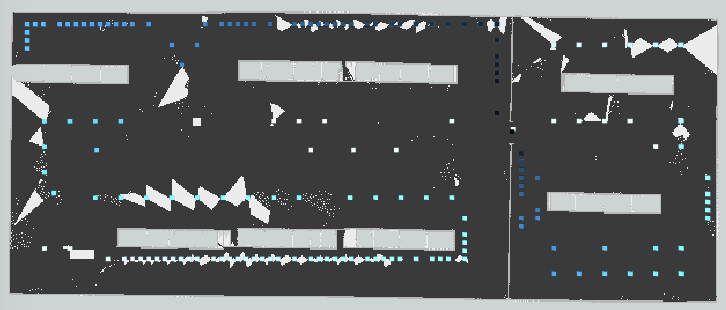
\includegraphics[width=0.9\textwidth]{./images/chapter5/warehouse_4_wall_follow_sampling_without_inloop_elim.png}
    \caption{Παράδειγμα Πεδίου Εκτίμησης Κάλυψης με Διαγραφή Περιττών Σημείων}
    \label{fig:coverage_estimation_ogm_with_elimination_example}
\end{figure}



\begin{algorithm}[H]
\caption{A Priori Coverage}
\label{alg:a_priori_coverage}
\begin{algorithmic}[1]
    \Function{aPrioriCoverage}{ogm, brushfire, nodes, eliminate, resolution, sensor\_range, sensor\_fov, sensor\_direction}
    \State $coverage = numpy.zeros(ogm.shape)$
    \State $new\_nodes = []$
    \For{$room$ in $nodes$}
        \State $new\_room = []$
        \For{$i$ in $range(len(room))$}
            \State $x, y = room[i]['position']$, $yaw = room[i]['yaw']$
            \If{not $i$ or $i == len(room)-1$ or not $eliminate$}
                \State $coverage$, $previous\_robot\_pose =  updateCover($ \par
                \hskip \algorithmicindent $room[i-1]['position'], ogm, coverage, resolution, sensor\_range, $ \par
                \hskip \algorithmicindent $sensor\_fov, sensor\_direction)$
                \State $updated = $True
            \Else
                \State $updated$, $coverage = checkAndUpdateCover(brushire, 0.85, ogm, coverage,$\par 
                \hskip\algorithmicindent $ resolution, sensor\_range, sensor\_fov, sensor\_direction)$
            \EndIf
            \If{$updated$}
                \State $new\_room.append(room[i])$
            \EndIf
        \EndFor
        \State $new\_nodes.append(new\_room)$
        \State $i++$
    \EndFor
    \State \Return $new\_nodes$
\end{algorithmic}
\end{algorithm}



\begin{algorithm}[H]
\caption{Check And Update Cover}
\label{alg:check_and_update_cover}
\begin{algorithmic}[1]
    \Function{checkAndUpdateCover}{brushfire, threshold, ogm, coverage, resolution,  sensor\_range, sensor\_fov, sensor\_direction}
    \State Read robot's pose $xx$, $yy$, $th$
    \State $indexes = []$
    \For{each sensor $s$}
        \State $cover\_length = int(sensor\_range[s] / resolution)$
        \State $temp = circularRayCastCoverage((xx,yy), ogm, cover\_length, sensor\_fov[s],$\par
        \hskip\algorithmicindent $th, sensor\_direction[s])$
        \State $indexes.extend(temp)$
    \EndFor
    \State Compute percentage $perc$ of already covered points of $indexes$
    \State $updated = $False
    \If{$perc < threshold$}
        \State $updated = $True
        \For{$x$, $y$ in $indexes$}
            \State $coverage[x, y] = 100$
        \EndFor
    \EndIf
    \State \Return $updated$, $coverage$
\end{algorithmic}
\end{algorithm}

\subsection{Δημιουργία Αλληλουχίας Κόμβων Ζιγκ-Ζαγκ}
\label{subsection:zig_zag_sequence_implementation}

Το τελευταίο μέρος της υλοποίησης του συστήματος περιέχει την δημιουργία της δεύτερης στρατηγικής πλοήγησης στον χώρο. Αυτή είναι η πλοήγηση με κινήσεις σε μορφή ζιγκ ζαγκ. Η κίνηση του οχήματος χρησιμοποιώντας αυτή την στρατηγική έχει δύο πλεονεκτήματα. Πρώτον, κάθε εμπόδιο θα σαρώνεται περισσότερες φορές και, δεύτερον, οι σαρώσεις θα πραγματοποιούνται με διαφορετικές γωνίες μεταξύ αισθήρα και εμποδίου, προσφέροντας πιο αναλυτική και ομοιόμορφη κάλυψη. Στην ιδανική περίπτωση στόχος είναι να σαρωθεί ένα εμπόδιο τόσο από το θετικό μισό τόξο του αισθητήρα, όσο και από το αρνητικό \ref{fig:different_angle_cover_example}. Βέβαια, όσες περισσότερες φορές και υπό διαφορετικές γωνίες σαρώσουν οι αισθητήρες ένα σημείο, τόσο πιο βέβαιο θα είναι το αποτέλεσμα. Το σημαντικό μειονέκτημα, όμως, της περίπτωσης αυτής είναι η αύξηση του συνόλου των στόχων που έχει να προσεγγίσει το όχημα και, επομένως, η αύξηση του συνολικού χρόνου κάλυψης του χώρου.

Ένας πολύ απλός και ταυτόχρονα αποτελεσματικός τρόπος παραγωγής μιας τέτοιας πορείας είναι η προσθήκη σημείων στόχων στην ήδη υπάρχουσα βέλτιστη ακολουθία, με στόχο την δημιουργία ζιγκ ζαγκ κινήσεων. Η προσθήκη τέτοιων στόχων μεταξύ των συνεχώμενων γειτονικών σημείων με μια μικρή απόκλιση από την μεταξύ τους ευθεία θα επιφέρει το επιθυμητό αποτέλεσμα. Ο αλγόριθμος αυτός παρουσιάζεται στο \ref{alg:add_zig_zag_nodes} και αναλύεται στη συνέχεια. Η ακολουθία κάθε δωματίου εξετάζεται χωριστά. Τα ήδη υπολογισμένα σημεία διατηρούνται ανέπαφα και ενδιάμεσα τους προστίθενται νέα, όπου κρίνεται απαραίτητο. Η διαδικασία εκμεταλλεύεται το γεγονός ότι η δειγματοληψία που έχει υλοποιηθεί έχει σταθερά βήματα, συνεπώς είναι εύκολα διακριτό εαν δύο σημεία βρίσκονται πολύ κοντά και χρίζουν προσθήκης νέων ενδιάμεσων στόχων. Θα έχουν μια από τις δύο μεταβλητές θέσης ίσες, πράγμα δεδομένο λόγω της ομοιόμορφης δειγματοληψίας σε κάθε βήμα. Εαν ισχύει αυτό και τα δύο σημεία είναι αρκετά κοντά, αλλά δεν ταυτίζονται, τότε προστίθεται ένας ακόμη στόχος. Υπολογίζεται η μέση των δύο σημείων και η απόσταση του νέου σημείου από την ευθεία τους η οποία είναι η μισή από την μεταξύ τους απόσταση, ώστε η τροχιά του οχήματος να είναι όσο πιο ομαλή γίνεται. Από τις δύο υποψήφιες θέσεις επιλέγεται αυτή με μεγαλύτερη τιμή brushfire, καθώς θα απέχει μεγαλύτερη απόσταση από τα εμπόδια. Έπειτα, καθώς κάθε στόχος περιέχει και τον προσανατολισμό του οχήματος, τίθεται ως τιμή στροφής του οχήματος η γωνία της ευθείας μεταξύ του τρέχοντος σημείου και του νέου, κάτι που δεν θα επηρεάζει, δηλαδή, τη συνολική κίνηση του οχήματος. Τέλος προκειμένου, να προστεθεί στην αλληλουχία το νέο σημείο πρέπει να ανήκει στο εν λόγω δωμάτιο, γι αυτό και πραγματοποιείται ο αντίστοιχος έλεγχος. 

Η διαδικασία οπτικοποιείται στο \ref{fig:example_zig_zag_choice}. Τα κόκκινα σημεία έχουν βρεθεί μέσω της δειγματοληψίας και είναι πολύ κοντά, συνεπώς μπορεί να προστεθεί ένας ακόμη στόχος ενδιάμεσα τους για να προκληθεί η ζιγκ ζαγκ κίνηση. Η ευθεία των σημείων σημειώνεται με πράσινο. Τα μπλε σημεία είναι τα δύο υποψήφια να προστεθούν στην ακολουθία, τα οποία βρίσκονται πάνω στην μεσοκάθετο του ευθύγραμμου τμήματος των δύο σημείων. Επιλέγεται, τελικά, αυτό που απέχει την μεγαλύτερη απόσταση από τα γύρω εμπόδια, δηλαδή το κάτω σημείο, το οποίο και έχει κυκλωθεί. Ένα παράδειγμα ζιγκ ζαγκ κίνησης μπροστά από ένα εμπόδιο είναι το \ref{fig:example_zig_zag_path}.


\begin{figure}[!htb]
    \centering
    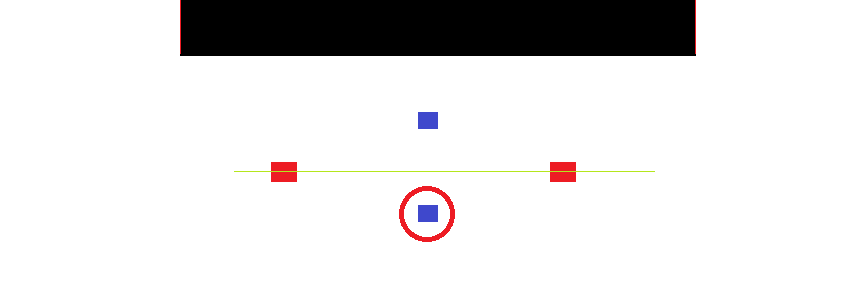
\includegraphics[width=0.8\textwidth]{./images/chapter5/example_zig_zag_choice.png}
    \caption{Παράδειγμα Επιλογής Ζιγκ Ζαγκ Σημείου}
    \label{fig:example_zig_zag_choice}
\end{figure}




\begin{figure}[!htb]
    \centering
    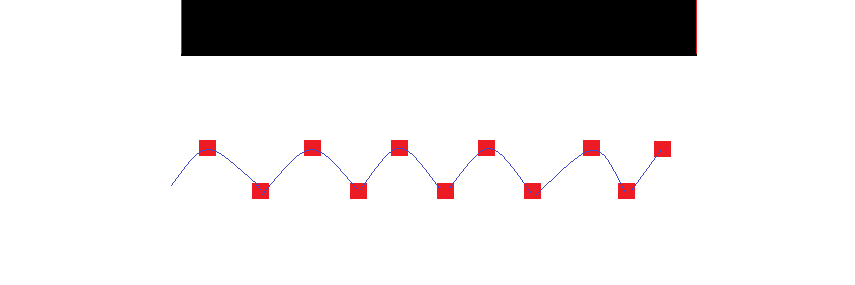
\includegraphics[width=0.8\textwidth]{./images/chapter5/example_zig_zag_path.png}
    \caption{Παράδειγμα Κίνησης Ζιγκ Ζαγκ παράλληλα με ένα εμπόδιο}
    \label{fig:example_zig_zag_path}
\end{figure}


\begin{algorithm}[H]
\caption{Add Zig Zag Nodes}
\label{alg:add_zig_zag_nodes}
\begin{algorithmic}[1]
    \Function{addZigZagNodes}{sequence, brushfire, ogm, sensor\_range, resolution}
        \State $zig\_zag\_sequence = []$
        \For{each $room$ in $sequence$}
            \State $temp\_sequence = []$
            \For{$i$ in $range(len(room))$}
                \If{not $i$}
                    \State $temp\_sequence.append(room[i])$
                    \State continue
                \EndIf
                \State $node = room[i]['position']$, $previous\_node = room[i-1]['position']$
                \State $x\_final, y\_final = 0, 0$
                \If{$previous\_node[0] == node[0]$ and $abs(previous\_node[1]-node[1])$ and $abs(previous\_node[1]-node[1]) <= max(sensor\_range)/ resolution$}
                    \State $dif = abs(previous\_node[1]-node[1])$
                    \State $x1 = int(node[0] - dif/2)$, $x2 = int(node[0] + dif/2)$
                    \State $y = int(min([previous\_node[1],node[1]]) + dif/2)$
                    \If{$brushfire[x1,y] >= brushfire[x2,y]$}
                        \State $x\_final = x1$, $y\_final = y$, $yaw = math.degrees(math.atan2(y-node[1], x1-node[0]))$
                    \Else
                         \State $x\_final = x2$, $y\_final = y$, $yaw = math.degrees(math.atan2(y-node[1], x2-node[0]))$
                    \EndIf
                \ElsIf{$previous\_node[1] == node[1]$ and $abs(previous\_node[0]-node[0])$ and $abs(previous\_node[0]-node[0]) <= max(sensor\_range)/resolution$}
                    \State $dif = abs(previous\_node[0]-node[0])$
                    \State $y1 = int(node[1] - dif/2)$, $y2 = int(node[1] + dif/2)$
                    \State $y = int(min([previous\_node[0],node[0]]) + dif/2)$
                    \If{$brushfire[x,y1] >= brushfire[x,y2]$}
                        \State $x\_final = x$, $y\_final = y1$, $yaw = math.degrees(math.atan2(y1-node[1], x-node[0]))$
                    \Else
                         \State $x\_final = x$, $y\_final = y2$, $yaw = math.degrees(math.atan2(y2-node[1], x-node[0]))$
                    \EndIf
                \EndIf
                \If{$(x\_final,y\_final)$ is point of $room$}
                    \State $temp\_sequence.append({'position': (x\_final,y\_final), 'yaw': yaw})$
                \EndIf
                \State $temp\_sequence.append(room[i])$
            \EndFor
            \State $zig\_zag\_sequence.append(temp\_sequence)$
        \EndFor
        \State \Return $zig\_zag\_sequence$
\end{algorithmic}
\end{algorithm}